% Taken from: https://mikedewar.wordpress.com/2009/02/25/latex-beamer-python-beauty/
\documentclass[12pt,english,pdf,xcolor=dvipsnames,aspectratio=169,handout]{beamer}\usepackage[]{graphicx}\usepackage[]{xcolor}
% maxwidth is the original width if it is less than linewidth
% otherwise use linewidth (to make sure the graphics do not exceed the margin)
\makeatletter
\def\maxwidth{ %
  \ifdim\Gin@nat@width>\linewidth
    \linewidth
  \else
    \Gin@nat@width
  \fi
}
\makeatother

\definecolor{fgcolor}{rgb}{0.345, 0.345, 0.345}
\newcommand{\hlnum}[1]{\textcolor[rgb]{0.686,0.059,0.569}{#1}}%
\newcommand{\hlstr}[1]{\textcolor[rgb]{0.192,0.494,0.8}{#1}}%
\newcommand{\hlcom}[1]{\textcolor[rgb]{0.678,0.584,0.686}{\textit{#1}}}%
\newcommand{\hlopt}[1]{\textcolor[rgb]{0,0,0}{#1}}%
\newcommand{\hlstd}[1]{\textcolor[rgb]{0.345,0.345,0.345}{#1}}%
\newcommand{\hlkwa}[1]{\textcolor[rgb]{0.161,0.373,0.58}{\textbf{#1}}}%
\newcommand{\hlkwb}[1]{\textcolor[rgb]{0.69,0.353,0.396}{#1}}%
\newcommand{\hlkwc}[1]{\textcolor[rgb]{0.333,0.667,0.333}{#1}}%
\newcommand{\hlkwd}[1]{\textcolor[rgb]{0.737,0.353,0.396}{\textbf{#1}}}%
\let\hlipl\hlkwb

\usepackage{framed}
\makeatletter
\newenvironment{kframe}{%
 \def\at@end@of@kframe{}%
 \ifinner\ifhmode%
  \def\at@end@of@kframe{\end{minipage}}%
  \begin{minipage}{\columnwidth}%
 \fi\fi%
 \def\FrameCommand##1{\hskip\@totalleftmargin \hskip-\fboxsep
 \colorbox{shadecolor}{##1}\hskip-\fboxsep
     % There is no \\@totalrightmargin, so:
     \hskip-\linewidth \hskip-\@totalleftmargin \hskip\columnwidth}%
 \MakeFramed {\advance\hsize-\width
   \@totalleftmargin\z@ \linewidth\hsize
   \@setminipage}}%
 {\par\unskip\endMakeFramed%
 \at@end@of@kframe}
\makeatother

\definecolor{shadecolor}{rgb}{.97, .97, .97}
\definecolor{messagecolor}{rgb}{0, 0, 0}
\definecolor{warningcolor}{rgb}{1, 0, 1}
\definecolor{errorcolor}{rgb}{1, 0, 0}
\newenvironment{knitrout}{}{} % an empty environment to be redefined in TeX

\usepackage{alltt}
\usepackage{etex}
\usetheme{default}
\beamertemplatenavigationsymbolsempty
\definecolor{fore}{RGB}{43,41,46}
\definecolor{back}{RGB}{255,255,255}
\definecolor{title}{RGB}{198,24,38}
\setbeamercolor{titlelike}{fg=title}
\setbeamercolor{normal text}{fg=fore,bg=back}
\usepackage{mathpazo}
\usepackage{amsmath}
\usepackage{multirow}
\renewcommand{\familydefault}{\rmdefault}
\usepackage[T1]{fontenc}
\usepackage{inputenc}
\usepackage{parskip}
\setcounter{secnumdepth}{3}
\setcounter{tocdepth}{3}
\usepackage{hyperref}
\hypersetup{pdfauthor={Constantin Manuel Bosancianu},
pdftitle={Advanced Topics in Applied Regression},
pdfsubject={Day 2: Heteroskedasticity and Its Solutions},
pdfkeywords={Budapest, ECPR, 2017, day 2, SSMT}}
\usepackage{babel}
\usepackage{graphicx}
\usepackage{subfigure}
\usepackage{palatino}
% Defines a checkmark
\def\checkmark{\tikz\fill[scale=0.4,color=title](0,.35) -- (.25,0) -- (1,.7) -- (.25,.15) -- cycle;}
\setbeamertemplate{itemize items}{\checkmark}
% For table captions in Beamer
\usepackage[labelformat=empty]{caption}
\captionsetup[figure]{labelfont={color=fore}}
\captionsetup[table]{labelfont={color=fore}}
\usepackage{tikz, tikz-cd, animate}
\usetikzlibrary{shapes,backgrounds,trees}
\usetikzlibrary{decorations.pathreplacing}
\usepackage{pgfplots}
\pgfplotsset{compat=1.10}
\usepgfplotslibrary{fillbetween}
\usepackage{pgfplotstable}
\usepackage{wrapfig}
\usepackage{booktabs}
\usepackage{dcolumn}
\usepackage[sectionbib]{apacite}
\renewcommand{\bibliographytypesize}{\footnotesize}
% Set the design of the footer
\makeatletter
\setbeamercolor{author in head/foot}{fg=white, bg=title}
\setbeamercolor{date in head/foot}{fg=white, bg=title}
\setbeamercolor{institute in head/foot}{fg=white, bg=title}
\setbeamertemplate{footline}
{
  \leavevmode%
  \hbox{%
  \begin{beamercolorbox}[wd=.3333333\paperwidth,ht=2.25ex,dp=1ex,center]{author in head/foot}%
    \usebeamerfont{author in head/foot}\insertauthor
  \end{beamercolorbox}%
    \begin{beamercolorbox}[wd=.3333333\paperwidth,ht=2.25ex,dp=1ex,center]{institute in head/foot}%
    \usebeamerfont{institute in head/foot}Central European University, Budapest
  \end{beamercolorbox}%
  \begin{beamercolorbox}[wd=.3333333\paperwidth,ht=2.25ex,dp=1ex,right]{date in head/foot}%
    \usebeamerfont{date in head/foot}\insertshortdate{}\hspace*{2em}
    \insertframenumber{} / \inserttotalframenumber\hspace*{2ex}
  \end{beamercolorbox}}%
  \vskip0pt%
}
\makeatother
\title{Advanced Topics in Applied Regression}
\subtitle{Day 2: Heteroskedasticity and Its Solutions}
\author{Constantin Manuel Bosancianu}
\institute{Doctoral School of Political Science \\ Central European University, Budapest\\\href{mailto:bosancianu@icloud.com}{bosancianu@icloud.com}}
\date{August 1, 2017}
\IfFileExists{upquote.sty}{\usepackage{upquote}}{}
\begin{document}
\maketitle
% PREAMBLE %
\section{Preamble}



\begin{frame}{Detour into definitions}

$a$, $b_1$, $e$ = estimates (based on the sample).\bigskip

$\alpha$, $\beta_1$, $\epsilon$ = parameters (in the population).\bigskip

Naturally, we can rarely know the parameters in the population; all we can do is reduce our uncertainty in guessing them based on the sample.\footnote{We're basically talking about 2 models: a theoretical one, and an empirical one.}

\end{frame}



\begin{frame}{OLS estimator: unbiasedness}

We're aiming for estimates to have a series of desirable properties. To begin with, in a finite sample:

\begin{itemize}
  \item Unbiasedness: $E(b)=\beta$ (we're not \textit{systematically} over- or under- estimating $\beta$);
\end{itemize}\bigskip

It can be shown with a substitution and about 4 lines of math that:

\begin{equation}
E(b) = \beta + E\left(\frac{\sum_{i=1}^n(x_i-\bar{X})(\epsilon_i - \bar{\epsilon})}{\sum_{i=1}^n(x_i - \bar{X})^2}\right)
\end{equation}

That fraction's top part is 0 if $E(\epsilon | X) = 0$.

\end{frame}



\begin{frame}{OLS estimator: efficiency}

Also in a finite sample:

\begin{itemize}
  \item Efficiency: $Var(b)$ is smaller than that of any other linear unbiased estimator;
\end{itemize}\bigskip

The proof here is a bit longer, but this variance of $b$ depends on the variance of $x$ and of the $e_i$.\bigskip

When this condition is not met, we call the estimator \textit{inefficient}.\footnote{The \textit{Gauss-Markov} theorem guarantees that under 3 assumptions (homoskedasticity, linearity, and error independence), OLS is efficient.}

\end{frame}



\begin{frame}{OLS estimator: normality}

As the sample grows to infinity (asymptotically), we can also expect to have:

\begin{itemize}
  \item Normality: the sampling distribution of $b$ will be centered on $\beta$, with known variance;
\end{itemize}\bigskip

\begin{equation}
b \sim \mathcal{N}\left(\beta, \frac{\sigma_e^2}{(n-1)\sigma_x^2}\right)
\end{equation}

This result\footnote{Does not require that $e_i \sim \mathcal{N}$. Needs the same 3 assumptions as for efficiency.} is important as it allows us to conduct significance tests, and then construct confidence intervals.

\end{frame}



\begin{frame}{OLS estimator: consistency}

This one is not mentioned very often. As sample grows to infinity, we want to see $b$ moving closer and closer to $\beta$.

\begin{equation}
\lim_{n\to\infty} P(|b - \beta|>\epsilon)=0,\quad \forall\; \epsilon > 0
\end{equation}

\texttt{BLUE}: OLS is a ``best linear unbiased estimator'' if assumptions hold.

\end{frame}


\section{Homoskedasticity}

\begin{frame}
\begin{center}
    \Huge Homoskedasticity
\end{center}
\end{frame}


\begin{frame}{Assumption of homoskedasticity}

\begin{equation}
Y_i = a + b_1X_{1i} + \dots + b_kX_{ki} + e_i
\end{equation}

This one targets the $e_i$, and specifically their variance---it must be constant, and not depend on any $X$s.

\begin{equation}
Var(e_i | X_1, \dots X_k) = \sigma_e^2
\end{equation}

Even when this assumption is violated, OLS estimates for $b$ are still unbiased, consistent, and asymptotically normal.\footnote{The bias depends on whether $E(\epsilon|x)=0$, not their variance.}

\end{frame}



\begin{frame}{Assumption of homoskedasticity}

However, in the presence of violations of homoskedasticity, the estimator loses its efficiency: $Var(b)$ is not as small as it could be.\bigskip

No amount of sample increase can solve this problem $\Rightarrow$ $t$-tests will be imprecise.\bigskip

\textit{Heteroskedasticity}: $Var(e_i) = h(X_1, \dots, X_k)$.\footnote{$h()$ is a generic function of the predictors in the model, either linear or nonlinear.}

\end{frame}



\section{Diagnosing heteroskedasticity}

\begin{frame}
\begin{center}
    \Huge Heteroskedasticity: diagnosis
\end{center}
\end{frame}


\begin{frame}{Ocular impact test}

Does it hit you right between the eyes when you plot it?



\begin{figure}
\centering
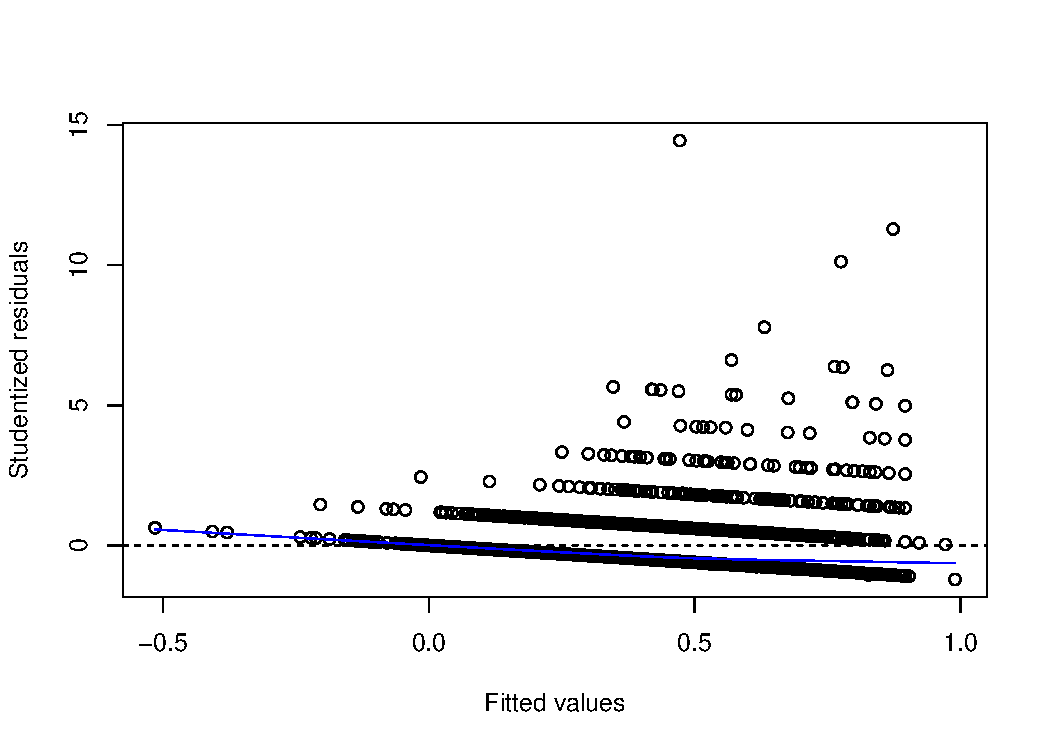
\includegraphics[scale=0.45]{../04-graphs/02-01}
\caption{Predicting \# of arrests in 1986}
\end{figure}

\end{frame}


\begin{frame}{Ocular impact test}



\begin{figure}
\centering
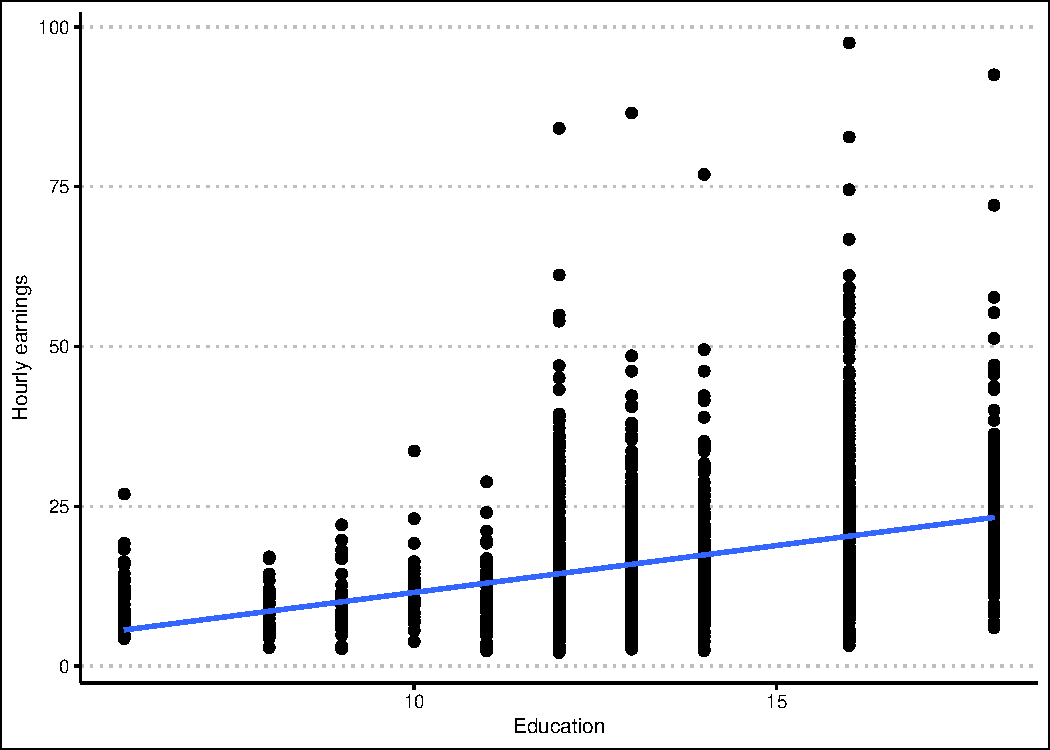
\includegraphics[scale=0.5]{../04-graphs/02-02}
\caption{Predicting earnings for 29--30 year olds in US (2004)}
\end{figure}

\end{frame}



\begin{frame}{Ocular impact test}




\begin{figure}
\centering
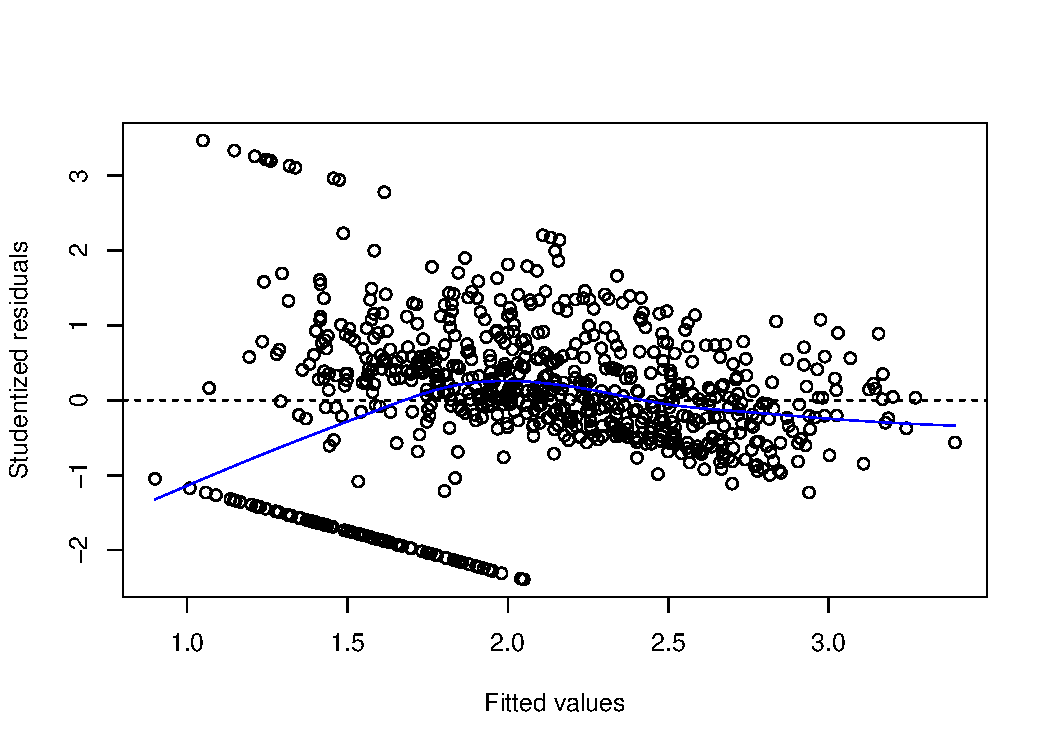
\includegraphics[scale=0.4]{../04-graphs/02-03}
\caption{Predicting students' GPAs in college}
\end{figure}

It can be effective, but only in the cases when there are glaring disparities between variances.
\end{frame}



\begin{frame}{Statistical tests: Breusch--Pagan (I)}

Take the standard form of the linear model:

\begin{equation}
Y_i = a + b_1X_{1i} + \dots + b_kX_{ki} + e_i
\end{equation}

The null hypothesis of the test is that $Var(e_i | X_1, \dots, X_k) = \sigma_e^2$.\bigskip

What we want to check is that there is no association between $e_i$, and any function that can be produced with the $X$s.

\end{frame}


\begin{frame}{Statistical tests: Breusch--Pagan (II)}

It's easiest to assume a linear form:

\begin{equation}
e_i^{\textcolor{title}{2}} = \delta_0 + \delta_1X_{1i} + \dots + \delta_kX_{ki} + \upsilon
\label{eq:eq-01}
\end{equation}

At this point, the last step is to just run an F test, or a Lagrange Multiplier test and check that $\delta_0=\delta_1=\dots=\delta_k=0$.\footnote{Technically, this second model would use $\epsilon_i$, but these cannot be known, so they get replaced with $e_i$.}\bigskip

This test is simply $LM=n \times R_*^2$, where $R_*^2$ is the model fit of the model in Equation \ref{eq:eq-01}, and $n$ is the sample size.

\end{frame}


\begin{frame}{Statistical tests: Breusch--Pagan (III)}

The value of the Breusch--Pagan test statistic (the LM from before) will have a $\chi^2$ distribution with $k$ degrees of freedom.\bigskip

If you wanted to, you could also construct an $F$-test, using the same $R_*^2$ value.

\begin{equation}
F = \frac{\frac{R_*^2}{k}}{(1-R_*^2)(n-k-1)}
\end{equation}

This will have a $F_{k, n-k-1}$ distribution.\footnote{You won't need to know critical values for these distributions, as the software will do it automatically for you.}

\end{frame}



\begin{frame}{Statistical tests: Breusch--Pagan (IV)}





\begin{figure}
\centering
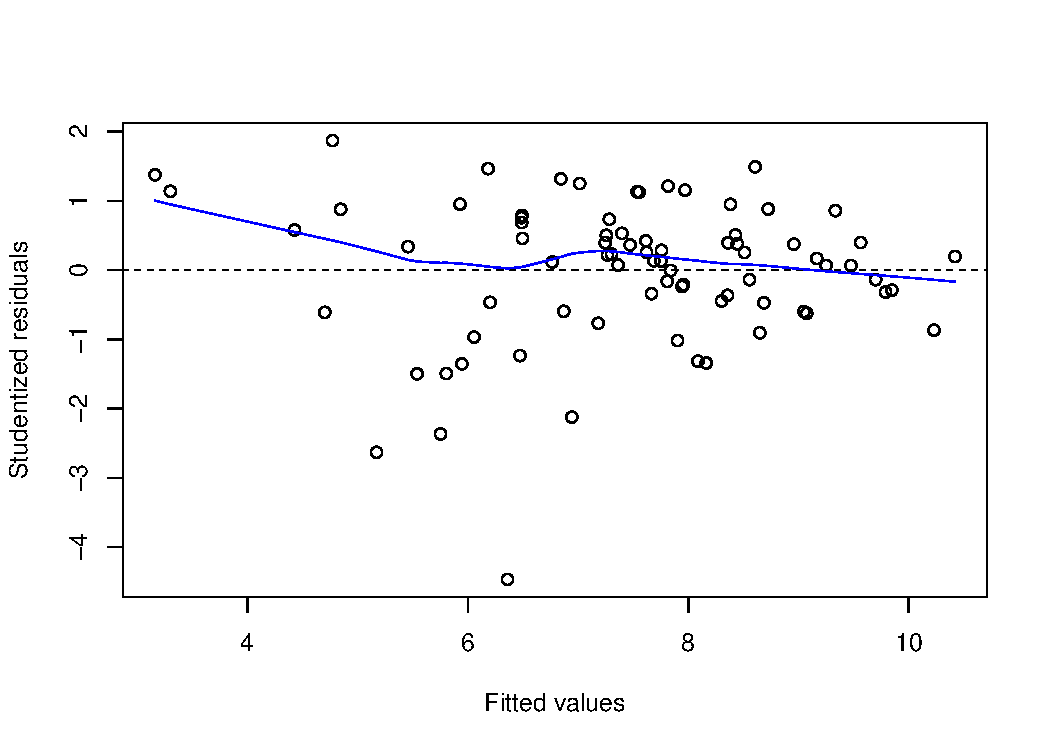
\includegraphics[scale=0.5]{../04-graphs/02-04}
\caption{Predicting GPA with IQ, gender, and self-concept}
\end{figure}

\end{frame}



\begin{frame}[fragile]{Statistical tests: Breusch--Pagan (V)}

\begin{knitrout}\footnotesize
\definecolor{shadecolor}{rgb}{0.969, 0.969, 0.969}\color{fgcolor}\begin{kframe}
\begin{alltt}
\hlkwd{bptest}\hlstd{(model1)} \hlcom{# requires the "lm" object}
\end{alltt}
\begin{verbatim}

	studentized Breusch-Pagan test

data:  model1
BP = 7.953, df = 3, p-value = 0.04699
\end{verbatim}
\end{kframe}
\end{knitrout}

The most important fact to remember is $H_0$ (!): homoskedasticity.\bigskip

In this case, we have to reject $H_0$ and accept that the data is heteroskedastic.

\end{frame}


\begin{frame}{Statistical tests: White}
  Not as common as Breusch--Pagan, although it shares a lot of similarities.\bigskip

  It adds to Equation \ref{eq:eq-01} all squares of the predictors, as well as all two-way interactions between predictors.\bigskip

  \begin{equation}
    \footnotesize
e_i^{\textcolor{title}{2}} = \delta_0 + \delta_1X_1 + \delta_2X_2 + \delta_3X_1^2 + \delta_4X_2^2 + \delta_5X_1X_2 + \upsilon
  \end{equation}

  It then proceeds either with an $F$-test or an LM test, as in the case of Breusch--Pagan.
  
\end{frame}


\begin{frame}{A final word of caution}
  Tests are very convenient, and authoritative for a readership, but there is a catch.\bigskip

  If there is a problem with the functional form of the model, $E(Y|X)$, then it might well be that the test reveals heteroskedasticity, when in fact none exists if the ``true'' model were used.\bigskip

  This was the case with yesterday's example with Boston house prices.
  
\end{frame}


\section{Solution: robust standard errors}

\begin{frame}
\begin{center}
    \Huge Solution I: Heteroskedasticity-robust SEs
\end{center}
\end{frame}


\begin{frame}{Robust SEs}
  We just concede that we don't know the form of $h(X_1, \dots, X_k)$ that explains $\sigma_e^2$.\bigskip

  However, we know that the only worrying problem with heteroskedasticity are the SEs, not $b$.\bigskip

  Robust SEs fix just that.\footnote{Also known as heteroskedasticity-robust, heteroskedasticity-consistent, sandwich estimators, cluster-robust etc.}

\end{frame}


\begin{frame}{Robust SEs -- simple regression}
  \citeA{white1980} shows how to obtain a valid estimator of $Var(b)$ even in conditions of heteroskedasticity.\bigskip

  \begin{equation}
V(b) = \frac{\sigma_e^2}{\sum_{i=1}^n(x_i - \bar{x})^2} = \frac{\sum_{i=1}^n[(x_i-\bar{X})^2\sigma_e^2]}{[\sum_{i=1}^n(x_i-\bar{X})^2]^2}
\end{equation}

In cases of heteroskedasticity, there is no more constant $\sigma_e^2$, but a variable $\sigma_i^2$.

The top part no longer simplifies nicely with a variable $\sigma_i^2$.

\end{frame}


\begin{frame}{Robust SEs -- simple regression}
  However, the following modification \textit{is} valid:

  \begin{equation}
V(b) = \frac{\sum_{i=1}^n[(x_i-\bar{X})^2e_i^2]}{[\sum_{i=1}^n(x_i-\bar{X})^2]^2}
\end{equation}

The square root of this quantity will be the heteroskedasticity-consistent SE.\footnote{The bottom part of that fraction looks scary, but it's really the square of the total sum of squares: $SST_x^2$.}

\end{frame}


\begin{frame}{Robust SEs -- multiple regression}

  \begin{equation}
V(b) = \frac{\sum_{i=1}^n(r_{ij}^2e_i^2)}{SST_j(1-R_j^2)}
\end{equation}

\begin{itemize}
\item $r_{ij}$: the $i$th residual from a regression of $X_j$ on all other predictors;
\item $SST_j$: the total sum of squares of $X_j$;
\item $R_j^2$: the $R^2$ from the regression of $X_j$ on all other predictors.
\end{itemize}

\end{frame}


\begin{frame}{Robust $F$-test and $LM$ test}

They can be computed, although for $F$-tests the formula does not have a simple form.\bigskip

An $LM$ test is simpler to conduct. Say that you have a full model

\begin{equation}
  Y_i = a + b_1X_1 + b_2X_2 + b_3X_3 + e_i
\end{equation}

and a restricted model

\begin{equation}
  Y_i = a + b_1X_1 + u_i
\end{equation}

\end{frame}



\begin{frame}{Robust $LM$ test (I)}

  The goal is to see whether $b_2=b_3=0$.\bigskip

  First, take out the $u_i$ from the restricted model.\bigskip

  Second, regress $X_2$ on $X_1$, and take out residuals $w1_i$. Also regress $X_3$ on $X_1$, and take out residuals $w2_i$.\footnote{If the restricted model would have had more predictors, we would have regressed $X_2$, and then $X_3$, on all these predictors.}\bigskip

  Third, compute $u_iw1_i$, and $u_iw2_i$ (and more products if we had more residuals from stage 2).

\end{frame}


\begin{frame}{Robust $LM$ test (II)}

  Finally, run this regression (notice there is no intercept):

\begin{equation}
  1 = \gamma_1u_iw1_i + \gamma_2u_iw2_i + \upsilon
\label{eq:eq-2}
\end{equation}  

Then $LM = n - SSR_1$, where $n$ is the sample size and $SSR_1$ is the sum of squared residuals from the regression in Equation \ref{eq:eq-2}.\bigskip

The $LM$ test statistic will have a $\chi^2$ distribution with $q$ degrees of freedom, where $q$ is the number of restrictions we imposed (here $q=2$).

\end{frame}


\section{Solution: WLS}

\begin{frame}
\begin{center}
    \Huge Solution II: Weighted Least Squares
\end{center}
\end{frame}


\begin{frame}{Weighted Least Squares}
  Suitable for when we can specify the functional form of the heteroskedasticity.\bigskip

  We can do this either by knowing the form beforehand (theory, studies), or by estimating it from the data itself.\bigskip

  If this is possible, WLS is more efficient than OLS in conditions of heteroskedasticity.
\end{frame}


\begin{frame}{WLS I: simple version}



\begin{figure}
\centering
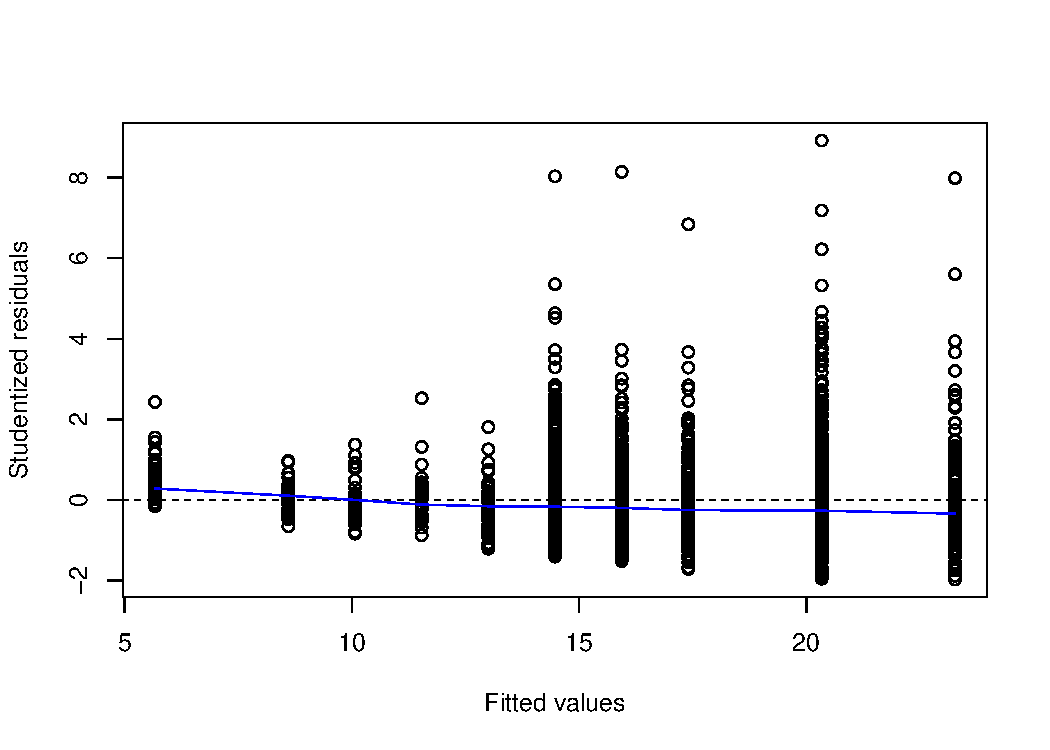
\includegraphics[scale=0.45]{../04-graphs/02-05}
\end{figure}

Say that $Var(e_i|educ) = \sigma_e^2h(educ)$, and that in this case $h(educ)=educ$.\footnote{I call this function $h_i$ from now on, to simplify notation.}

\end{frame}


\begin{frame}{WLS I: simple version}
 Even though the variance of $e_i$ is not constant, it turns out that the variance of $\frac{e_i}{\sqrt{h_i}}$ is constant and equal to $\sigma_e^2$.\bigskip

   This means we can use the $\frac{1}{\sqrt{h_i}}$ quantity as a weight, and re-specify the model of earnings.

   \begin{equation}
     \footnotesize
     Earn_i/\sqrt{educ_i} = a/\sqrt{educ_i} + b_1\underbrace{educ_i/\sqrt{educ_i}}_{=\sqrt{educ_i}} + \underbrace{e_i/\sqrt{educ_i}}_{e_i^*}
   \end{equation}

   The new errors, $e_i^*$ are homoskedastic, with 0 conditional expectation.
 \end{frame}


 \begin{frame}{WLS I: simple version}
   The new coefficients from this respecified model, $a^*$, $b_1^*$, \dots, $b_k^*$ are GLS (generalized least squares) estimators.\bigskip

   They are more efficient than OLS estimators in this instance.\bigskip

   In practice, this procedure doesn't weight the variables themselves, but rather the $e_i^2$. The weights used are $\frac{1}{h_i}$. This means less weight is given to errors with higher variance.
 \end{frame}


 \begin{frame}[fragile]{Earnings specification}

\begin{table}
\caption{Model comparisons: OLS and GLS}
\begin{center}
\begin{scriptsize}
\begin{tabular}{l D{.}{.}{4.6} D{.}{.}{4.6} D{.}{.}{6.6}}
\toprule
 & \multicolumn{1}{c}{OLS} & \multicolumn{1}{c}{GLS} & \multicolumn{1}{c}{GLS through REML} \\
\midrule
(Intercept)    & -3.134^{**} & -1.823^{*}  & -1.823^{*}  \\
               & (0.959)     & (0.840)     & (0.840)     \\
Education      & 1.467^{***} & 1.370^{***} & 1.370^{***} \\
               & (0.070)     & (0.063)     & (0.063)     \\
\midrule
R$^2$          & 0.130       & 0.138       &             \\
Adj. R$^2$     & 0.130       & 0.138       &             \\
Num. obs.      & 2950        & 2950        & 2950        \\
AIC            &             &             & 21032.547   \\
BIC            &             &             & 21050.514   \\
Log Likelihood &             &             & -10513.274  \\
\bottomrule
\multicolumn{4}{l}{\tiny{$^{***}p<0.001$; $^{**}p<0.01$; $^{*}p<0.05$}}
\end{tabular}
\end{scriptsize}
\label{table:coefficients}
\end{center}
\end{table}

\end{frame}


 \begin{frame}{WLS II: slightly more complex}

   In case you don't have information about a clear function for the variance, you can always try estimating it.\bigskip

   \begin{equation}
     Var(e_i|X_1,\dots,X_k) = \sigma_e^2exp(\delta_0 + \delta_1X_1 + \dots + \delta_kX_k)
   \end{equation}

   The exponential function is preferred because it makes sure that the weights will always be positive.\footnote{A linear specification would not insure this by default. $exp(a)=e^a$, where $e$ is Euler's constant $\approx 2.71828$.}

   \begin{equation}
     log(e^2) = \alpha + \delta_1X_1 + \dots + \delta_kX_k + \upsilon
     \label{eq:eq-03}
   \end{equation}
 \end{frame}


 \begin{frame}{FGLS}
   From Equation \ref{eq:eq-03} all we need are the fitted values: $\hat{e_i}$.\bigskip

   Then we simply use $\frac{1}{exp(\hat{e_i})}$ as the weights in the original regression.\bigskip

   Using the same data to estimate both weights and the model, means that FGLS estimates are not unbiased, but they are asymptotically consistent and more efficient than OLS.

 \end{frame}


 \begin{frame}{WLS: final considerations}
   If estimates from OLS and WLS differ considerably, then there is a bigger problem than heteroskedasticity, e.g. perhaps model misspecification.\bigskip

   Getting the precise form of $h(x)$ right is not a big concern, as the estimates will still be consistent asymptotically.\bigskip

   With a wrong form of $h(x)$ there is no guarantee that WLS estimates are more efficient than OLS, but it's still better to use it than rely on OLS.
 \end{frame}



% FRAME
\begin{frame}
\begin{center}
    \Huge Thank \textcolor{title}{you} for the kind attention!
\end{center}
\end{frame}

% REFERENCES %

\begin{frame}
\frametitle{References}
\bibliographystyle{apacite}
\bibliography{../Bibliography}
\end{frame}

\end{document}
